\documentclass[a4paper,12pt, oneside]{article}

\title{\textbf{L'impatto del Codec AV1 sull'industria della visualizzazione online} \\ \large A.A 2023/2024 \\ Elaborato di Crittografia}
\author{Gabos Norbert \\ 0000970451 \\ tiberiunorbert.gabos@studio.unibo.it }
\date{}

\usepackage[T1]{fontenc}
\usepackage[utf8]{inputenc}
\usepackage[italian]{babel}
\pagestyle{plain}
\usepackage{graphicx}
\usepackage{hyperref}   % serve per i link
\hypersetup{
    colorlinks=true,
    linkcolor=blue,
    filecolor=magenta,      
    urlcolor=cyan,
    pdftitle={Overleaf Example},
    pdfpagemode=FullScreen,
}   % serve per i link
\usepackage[table,xcdraw]{xcolor}
\usepackage{tabularx}
\usepackage{ragged2e}               % migliora la formattazione del testo all'interno delle celle
\renewcommand{\arraystretch}{1.5}   % aggiunge margine alle celle
\graphicspath{{images/}}

\definecolor{darkBlue}{RGB}{21, 69, 179}
\definecolor{lightPink}{RGB}{242, 10, 172}

\begin{document}

\maketitle

\newpage
\tableofcontents{}
\newpage

\section{Introduzione}
Con l'avvento dei computer e la crescente digitalizzazione dei media, è emersa la necessità di
trovare soluzioni efficaci per rappresentare e archiviare i video all'interno dei sistemi
informatici. Questo processo ha comportato la trasformazione dei tradizionali filmati in una
forma compatibile con il mondo digitale, dove ogni istante del video è rappresentato da una
sequenza di immagini statiche, comunemente note come frame. Ogni frame, a sua volta, è
composto da una matrice di pixel, gli elementi fondamentali che compongono l'immagine, ognuno
dei quali è definito da una terna di colori \textbf{RGB} (Red, Green, Blue) e da una profondità
di colore che varia generalmente tra 0 e 255.

Questo approccio ha permesso di preservare la qualità visiva dei contenuti video e di renderli
compatibili con le capacità di elaborazione dei computer. Tuttavia, la mera rappresentazione
dei video in questo modo ha portato ad un'elevata quantità di dati da gestire ed archiviare
comportando sfide significative in termini di spazio di archiviazione e larghezza di banda.
Per esempio un banale video da 10 minuti in 1080p a 30 fotogrammi al secondo pesa
all'incirca 111 GB.
\noindent
\\\\Peso\_video = Risoluzione × Fotogrammi\_al\_secondo × Durata × Profondità\_colore\\

Nei primi anni '80, con il crescente bisogno di gestire file video in un contesto di limitate
capacità di archiviazione, si svilupparono i primi \textbf{codec} video. Questi non solo consentivano
la compressione dei file video, ma anche la decodifica. Questo rappresentava una soluzione
importante, poiché i dispositivi dell'epoca potevano immagazzinare solo una quantità limitata
di dati, mentre le esigenze di qualità video e il numero di dispositivi produttori di contenuti
multimediali aumentavano costantemente.
Per affrontare queste sfide e ottimizzare l'archiviazione e la trasmissione dei video
digitali, sono stati sviluppati una serie di algoritmi e standard di compressione video.
Esistono due approcci principali alla compressione video: la compressione \textbf{lossless} e
la compressione \textbf{lossy}. La compressione lossless, ad esempio con algoritmi come
\textbf{Huffyuv} e \textbf{Lagarith}, mira a ridurre le dimensioni del file senza perdita di
qualità, mantenendo ogni singolo dato originale. D'altro canto, la compressione lossy
sacrifica una certa quantità di qualità visiva per raggiungere una maggiore compressione dei
dati, consentendo una gestione più efficiente delle risorse di archiviazione e una
trasmissione più rapida attraverso le reti digitali.

In questa relazione, esploreremo l'evoluzione della compressione video lossy, partendo dal
contesto della sua necessità fino alla discussione di algoritmi più recenti e avanzati come il
Codec AV1. Analizzeremo come questi algoritmi hanno rivoluzionato il modo in cui i video
vengono elaborati, archiviati e trasmessi sui mezzi digitali, con un focus particolare sugli
impatti e le potenzialità di tali innovazioni nell'industria multimediale moderna.

\section{I primi passi}
\subsection{H.261}
Nel 1988 nasce il codec H261 che è stato il primo algoritmo di compressione video ad utilizzare
in modo efficiente degli algoritmo di \textbf{intraframe} e \textbf{interframe}, che sono
spiegati nel capitolo successivo, ed è responsabile dell'introduzione della codifica video
ibrida basata su blocchi, che è ancora utilizzata oggi in molti standard video.
\\\\Prima di proseguire, visto che non parliamo più dei video come una matrice di pixel, ma più di
un flusso di dati, bisogna introdurre il concetto di bitrate.
Il \textbf{bitrate} è una misura della velocità di trasmissione dei dati in un file multimediale,
come un video o un brano audio. Rappresenta quanti dati vengono trasmessi o elaborati in un
determinato intervallo di tempo espresso in \textbf{bit/s}. In generale, a parità di tecnologie
utilizzate per la compressione, più il bitrate di un contenuto è elevato e più la sua qualità
sarà maggiore al costo di un peso più elevato. Vedi Figura~\ref{fig:confronto_bitrate}.

\begin{figure}[h]
    \centering
    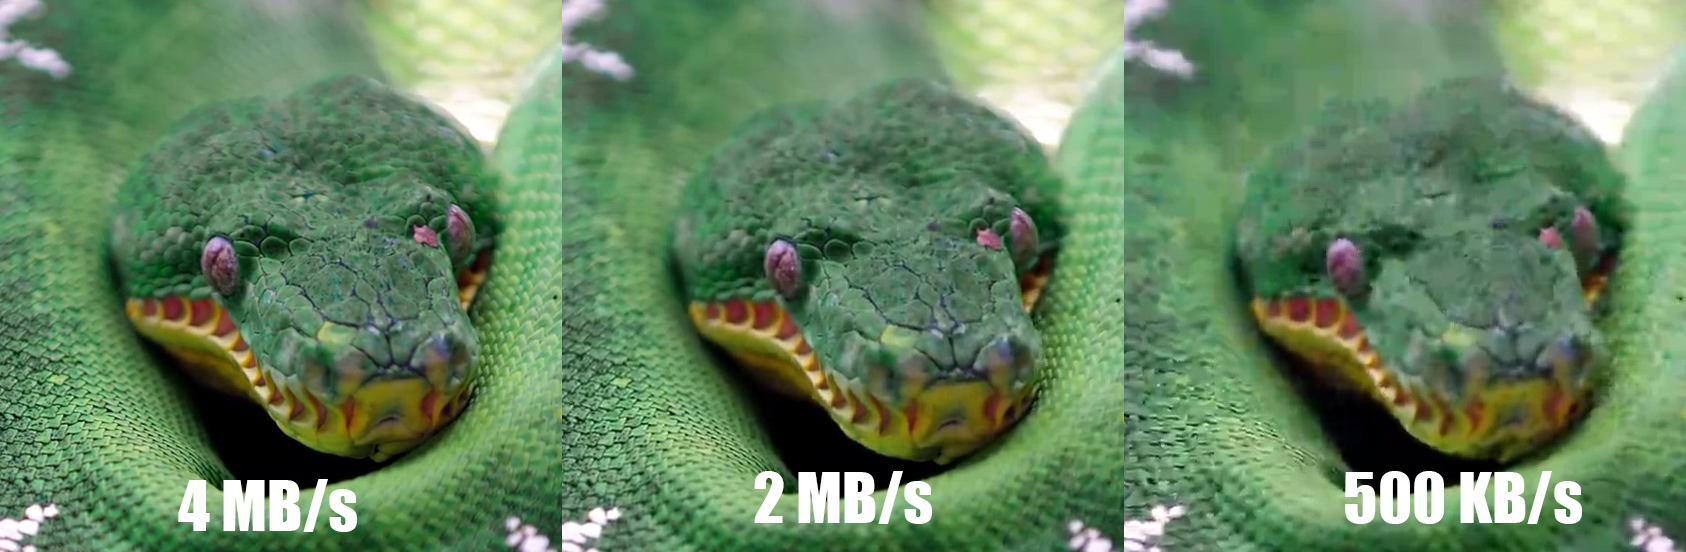
\includegraphics[width=1\textwidth]{images/confronto-bitrate.png}
    \caption{L'immagine mette a confronto 3 frame presi allo stesso istante da un video compresso con 3 valori di bitrate differenti.}
    \label{fig:confronto_bitrate}
\end{figure}

\noindent
Un aspetto sorprendente di questo algoritmo è che per rilevare una diminuzione nella qualità del
video, è necessario ridurre significativamente il bitrate.
Per fare un confronto con l'esempio di prima del video da 10 minuti, utilizzando questo codec potremmo
ridurre nettamente la dimensione del file anche di 300 volte. Usando un bitrate che varia dai 5-10 Mb/s,
quindi un bit rate elevato per questa risoluzione che ci permette di mantenere un'ottima qualità,
il file compresso avrebbe una dimensione dai 375 ai 750 MB.

\section{Tecnologie attuali}
TODO: Da qualche parte descrivere che cos'è Luma e Chroma
\subsection{H.264/AVC}
Il formato H.264 è stato introdotto nel 2003 e appartiene alla serie H.26X. Il suo obiettivo principale
è quello di comprimere ulteriormente i file video senza compromettere la qualità visiva. Questa
tecnologia consente di ottenere file video più leggeri mantenendo comunque un'elevata qualità
dell'immagine. In alternativa, è possibile mantenere le stesse dimensioni dei file video ma migliorare
la qualità visiva. Questo codec sarà fondamentale anche in futuro con l'espansione dei servizi di
streaming in tempo reale. Ciò permetterà alle aziende di risparmiare sui costi delle infrastrutture
per l'archiviazione e la trasmissione dei dati via rete, e offrirà agli utenti finali con connessioni
internet di scarsa qualità la possibilità di fruire di questi servizi.

Nonostante siano trascorsi più di 20 anni dalla creazione del formato H.264, merita comunque attenzione
in virtù del suo status di standard rivoluzionario nella codifica video. Nel settembre 2019, ha
raggiunto un notevole 91\% di adozione tra gli sviluppatori nel settore video, confermandosi così come
un pilastro fondamentale della tecnologia di compressione video. Inoltre, alcune delle tecnologie
adottate da questo codec saranno cruciali per comprendere meglio il funzionamento dei codec successivi.

\paragraph{Slices}\hphantom{A}\\
Una slice è una porzione sequenziale di dati all'interno di un frame video. Questa porzione è suddivisa
in unità più piccole chiamate macroblock. La divisione del frame in slice viene fatta per organizzare e
processare i dati video in modo efficiente durante la codifica e la decodifica. Un esempio di come
questo approccio potrebbe aumentare l'efficienza è quello di processare ogni slice con un thread diverso.

\paragraph{Macroblock}\hphantom{A}\\
Un immagine viene divisa in dei blocchi quadrati di pixel chiamati macroblock e possono avere una
dimensione variabile in base allo codec utilizzato, nel caso del H.264 è sempre 16x16 pixel. Il
macroblock non raggruppa al suo interno l'immagine originale, bensì 3 matrici più semplici, la
Luma e le matrici Cb e Cr della Chroma. Le dimensioni di queste sotto-matrici può variare da
formato a formato, ma nel caso del H.264 la Luma mantiene un la stessa dimensione dell'immagine
originale, ovvero 16x16, mentre le due matrici Cb e Cr, possono essere una campione 4x4, 8x4, 4x8.
Di solito il livello di campionamento delle matrici Chroma è inferiore a quella della Lume, in quanto
l'occhio umano è più attente ad osservare la luminosità e i bordi degli oggetti rispetto al colore.
Solo con questa piccola ottimizzazione si può risparmiare fino al 50\% sullo spazio occupato su disco.
Infine i macroblock possono essere suddivisi in blocchi più piccoli, chiamati
\textbf{prediction-blocks}, di vari dimensioni e forme, ad esempio il codec H.264 può suddividerli in
4 prediction-blocks da 8x8, oppure 16 da 1x1, ma esistono altri codec che possono suddividere i
macroblock in matrici rettangolari, oppure triangolari. Questa suddivisione in prediction-blocks
viene fatta in quanto un prediction-block più è piccolo e meglio riuscirà a rappresentare frammenti
di immagine che contengono molto dettaglio a discapito della potenza di calcolo necessaria a
decodificare l'immagine durante la fase di Intraframe. Si noti come nella
Figura~\ref{fig:macroblocks_sub_division}le regioni del cielo e della montagna, caratterizzate da
pixel simili, generino macroblocks più ampi. Al contrario, in zone in cui coesistono sia la montagna
che il cielo, i macroblocks sono più piccoli per gestire le variazioni nei dettagli di entrambe le
zone.

\begin{figure}[h]
    \centering
    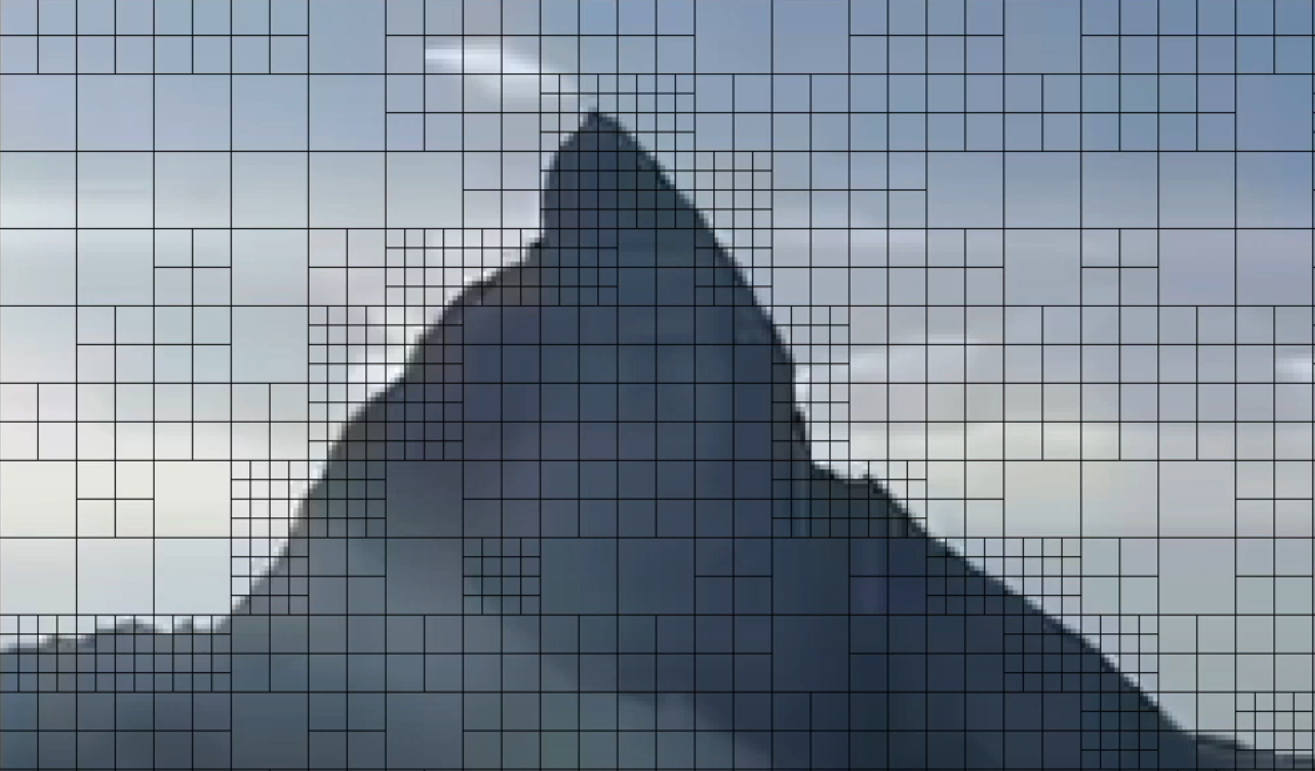
\includegraphics[width=1\textwidth]{images/macroblocks_sub-division.png}
    \caption{Suddivisione di un'immagine in macroblocks e prediction-blocks.}
    \label{fig:macroblocks_sub_division}
\end{figure}

TODO: volendo si possono inserire delle immagini per le slice e i macroblock

\paragraph{Intraframe/intra prediciton}\hphantom{A}\\
\begin{figure}[h]
    \centering
    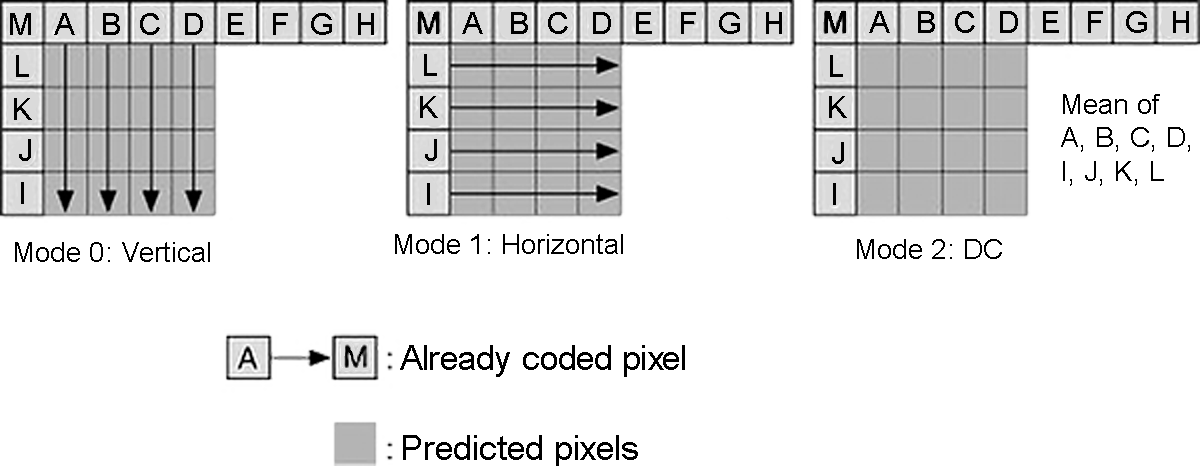
\includegraphics[width=1\textwidth]{images/intraframe-algo.png}
    \caption{Rappresentazione dei 3 metodi più utilizzati per la predizione intraframe}
    \label{fig:intraframe_algo}
\end{figure}
La compressione intraframe, si riferisce alla compressione dei dati all'interno di un singolo
fotogramma. Questo metodo si divide più passaggi:
\begin{enumerate}
  \item Per ogni macroblock o prediction-block, viene utilizzato un modello di predizione per stimare
  i valori delle matrici al suo interno basandosi sui valori delle celle adiacenti. Questo modello di
  predizione può essere semplice (es. facendo la media dei pixel adiacenti) o più complesso (come la
  predizione basata su modelli statistici o algoritmi di machine learning). I 3 metodi più utilizzati
  sono (Vedi Figura~\ref{fig:intraframe_algo}) : traslandolo i pixel adiacenti già noti in
  orizzontale/verticale oppure facendo una media dei pixel adiacenti.
  Nel caso del formato H.264 ci sono in totale 9 algoritmi di intraframe.
  \item Successivamente viene calcolata la residua, ovvero la differenza tra i pixel predetti e i
  pixel dell'immagine non compressa
  \item Infine viene scelta la matrice residua, che si è avvicinata di più al gruppo di pixel originale,
  comprimendo così la dimensione del frame.
\end{enumerate}
È nella fase di intraframe che viene fatta la suddivisione dei macroblock in prediction-block.
L'algoritmo sceglie la suddivisione migliore semplicemente provando tutti i tipi di divisioni dei
blocchi fino a trovare quello con la residua migliore.

TODO: non so se inserire l'esempio (nel caso le immagini sono gia salvate) (per rendere le idee piu chiare...)

\paragraph{Interframe/Motion compensation}\hphantom{A}\\
Quando si parla di compressione, l'obiettivo è ridurre al minimo le ridondanze. Nel contesto dei video,
si nota subito che frame adiacenti temporalmente condividono una considerevole quantità di pixel.
L'algoritmo di interframe si occupa proprio di questo aspetto. Invece di analizzare i singoli frame uno
dopo l'altro, prende in considerazione più frame contemporaneamente per individuare le similitudini tra
di essi. Naturalmente, ci sono situazioni in cui ciò non è fattibile, come durante un cambio di scena,
dove la maggior parte o addirittura tutti i pixel possono cambiare da un frame all'altro.

Per prima cosa se devono classificare ogni frame di un video, per fare ciò il video viene
ridimensionato ad una risoluzione inferiore e per ogni frame si applicano sia l'algoritmo di intraframe,
che di  interframe e si comparano i due risultati. Se il costo del intraframe è inferiore, questo
significa che il frame che si sta analizzando non ha elementi in comune con i frame precedenti,
suggerendo così un cambio di scena. Ci sono in totale 3 tipi di frame (vedi Figura~\ref{fig:frame_type}):

\begin{itemize}
  \item Il tipo \textbf{I frame} di solito indica un cambio di scena, pertanto si applica l'algoritmo
  di intraframe, poiché non ci sono altri frame di riferimento. Di conseguenza, questo è il frame meno
  compresso. 
  \item Il tipo \textbf{P frame} contiene solo la parte dell'immagine che è cambiata rispetto al fotogramma
  precedente o successivo, quindi si può applicare esclusivamente l'algoritmo di Interframe. Questo tipo di
  frame occupa circa il 50\% in meno di spazio rispetto al tipo I.
  \item Il tipo \textbf{B frame} è un ibrido tra i due precedenti, in quanto il frame corrente è un misto
  tra frame precedenti e successivi, ma che contiene elementi nuovi. Questo è il tipo di frame più
  efficiente in quanto occupa il 25\% dello spazio rispetto al tipo I.
\end{itemize}

\begin{figure}[h]
    \centering
    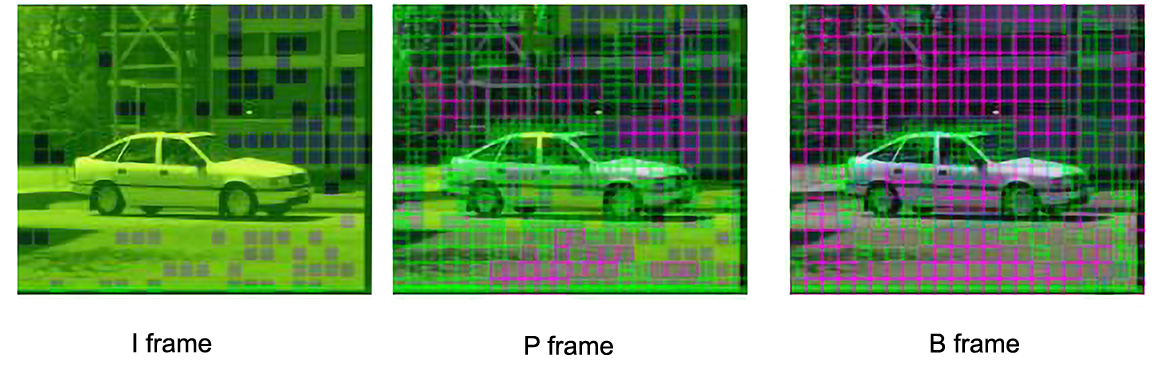
\includegraphics[width=1\textwidth]{images/frame-type.png}
    \caption{Classificazione del tipo di frame.
    I macroblock viola indicano che quel frame è stato ricostruito da un frame precedente,
    mentre quello verde che è stato codificato grazie ai pixel interni al frame.}
    \label{fig:frame_type}
\end{figure}

Nel dettaglio, per comprendere quali elementi di un frame vengono ripetuti all'interno di altri frame,
vengono nuovamente sfruttati i macroblock. Inoltre, i frame non vengono codificati in ordine cronologico,
ma in modo sparso, in modo che quando si analizza un frame che utilizza l'algoritmo di interframe, possa
attingere informazioni sia dai frame precedenti che da quelli successivi, come mostrato nella
Figura~\ref{fig:interframe}. Ci sono due modi per popolare un macroblock grazie al intraframe:

\begin{itemize}
  \item La \textbf{Uni-directional Motion Compensation} consiste nell'individuare il macroblock identico
  tra i frame precedenti o successivi e salvandolo come un \textbf{motion vector}, ovvero un vettore che
  identifica lo spostamento del macroblock tra i due frame.
  \item La \textbf{Bi-directional Motion Compensation} implica invece l'individuazione di due macroblock,
  uno nel frame successivo e uno in quello precedente, che più si avvicinano a quello in esame.
  Successivamente, si salvano i loro due motion vector e si combinano utilizzando una funzione matematica.
  Ad esempio, il codec H.264 calcola la media tra le due matrici, sottrae i pixel originali generando una
  matrice "residuo" e viene anch'essa memorizzata. Questo permette non solo di di memorizzare i
  macroblocks identici tra frame, ma anche di poter tracciare quelli che vengono ruotati, stirati o inclinati.
\end{itemize}

\begin{figure}[h]
    \centering
    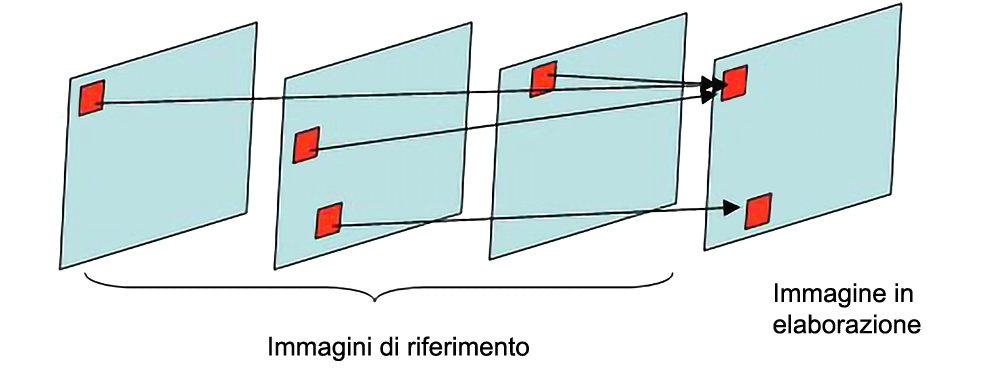
\includegraphics[width=1\textwidth]{images/interframe.png}
    \caption{Nella figura viene mostrato un esempio di come l'algoritmo di interframe
    attinge a frame diversi per ricostruire il macroblock interessato.}
    \label{fig:interframe}
\end{figure}

\paragraph{Transformation}\hphantom{A}\\
Ora che tutti i macroblocks sono stati in qualche modo codificati, si prendono solo quelli che contengono
dei residui e vengono divisi in blocchi rettangolari 8x8 e viene applicata la trasformata discreta del
coseno (\textbf{DCT} - Discrete Cosine Transform).

La trasformata discreta del coseno permette di rilevare variazioni di informazioni (come il colore per
i blocchi Chroma o la luminosità per i blocchi Lumen) trasformando i valori dei pixel dal dominio
spaziale al dominio delle frequenze individuando così i blocchi con con più dettagli, ovvero i blocchi
con frequenza maggiore.

Per applicare la trasformata discreta del coseno bisogna:

\begin{figure}[h]
    \centering
    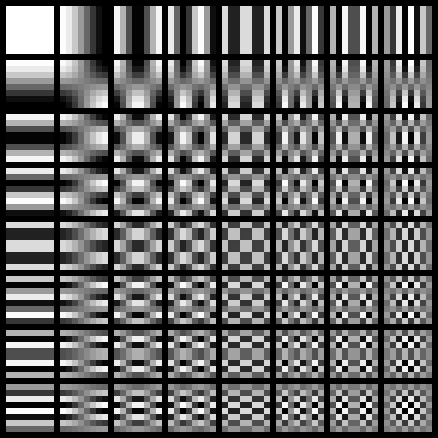
\includegraphics[width=0.8\textwidth]{images/DCT-table.png}
    \caption{Tabella DCT. In particolare si noti come partendo dall'angolo in alto a sinistra,
    più si va verso destra e più la frequenza della matrice aumenta in orizzontale e più si va
    verso il basso e più la frequenza della matrice aumenta in verticale.}
    \label{fig:DCT_table}
\end{figure}

\begin{enumerate}
    \item Dividere l'immagine (ovvero le 3 matrici dei residui) in piccoli blocchi quadrati 8x8
    \item Si normalizzano i valori delle matrici sottraendo a ciascun valore 128, cosi facendo
    ogni cella sarà compresa tra 128 e -127. Se prendiamo ad esempio la matrice Lumen il valore
    128 corrisponderà al bianco, mentre il valore -127 al nero e i valori centrali saranno tutte
    le tonalità di grigio
    \item Successivamente si cerca di ricostruire la matrice 8x8 ottenuta come somma di matrici
    prese da una matrice DCT precalcolata (vedi figura Figura~\ref{fig:DCT_table}. Nella 
    Figura~\ref{fig:DCT_example} si può notare come partendo da un immagine, come si possa
    risalire ad essa mediante una somma mi matrici prese dalla tabella DCT.
\end{enumerate}

\begin{figure}[h]
    \centering
    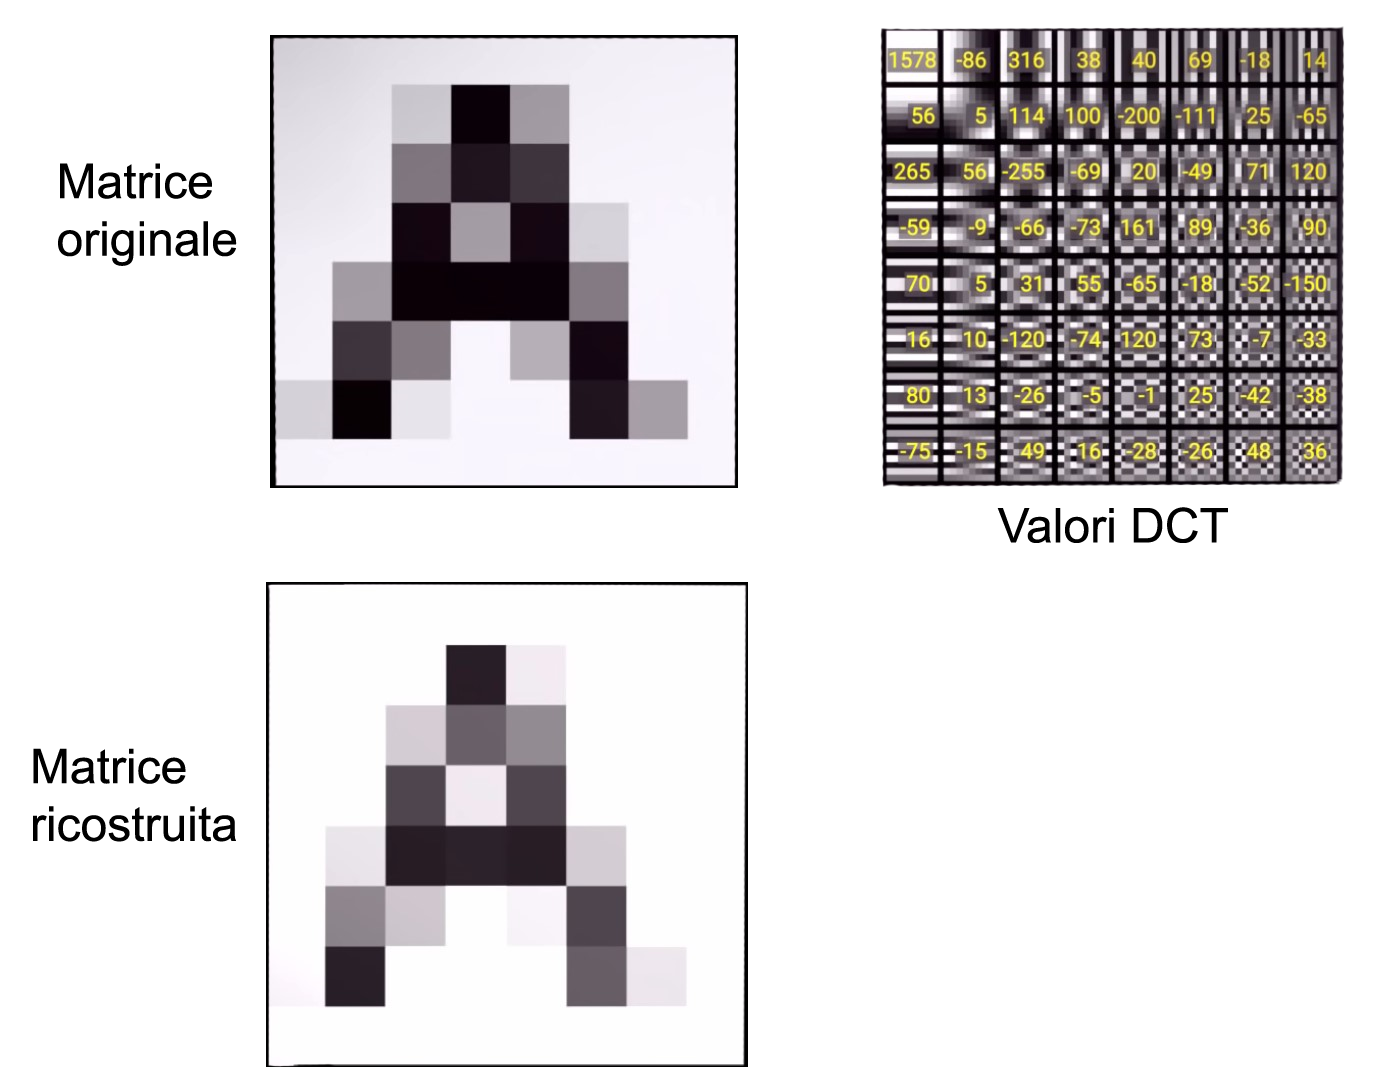
\includegraphics[width=1\textwidth]{images/DCT-example.png}
    \caption{Esempio di come una matrice (in alto a sinistra) mediante somma di matrici DCT
    più essere ricostruita.}
    \label{fig:DCT_example}
\end{figure}

\paragraph{Quantization}\hphantom{A}\\
La quantizzazione implica la creazione di due matrici, chiamate tabelle di quantizzazione, per
suddividere i valori delle matrici ottenute tramite la trasformazione. Queste due matrici, una
per le Luma e una per le Chroma, sono identiche per l'intera immagine e sono strutturate in
modo che i valori più elevati si trovino nella parte inferiore destra, corrispondente alle
frequenze più alte nell'immagine DCT. Questo schema favorisce una migliore compressione nelle
aree in cui le frequenze dell'immagine sono più elevate.

Per quantizzare un blocco, ogni valore DCT viene diviso per il valore corrispondente nella
tabella di quantizzazione e successivamente arrotondato al numero intero più vicino (vedi
l'esempio della Figura~\ref{fig:quantization_example}). Questo processo riduce leggermente la
qualità dell'immagine, ma lo fa in modo intelligente, rimuovendo dettagli dalle aree ad alta
frequenza, impercettibili per l'occhio umano.

\begin{figure}[h]
    \centering
    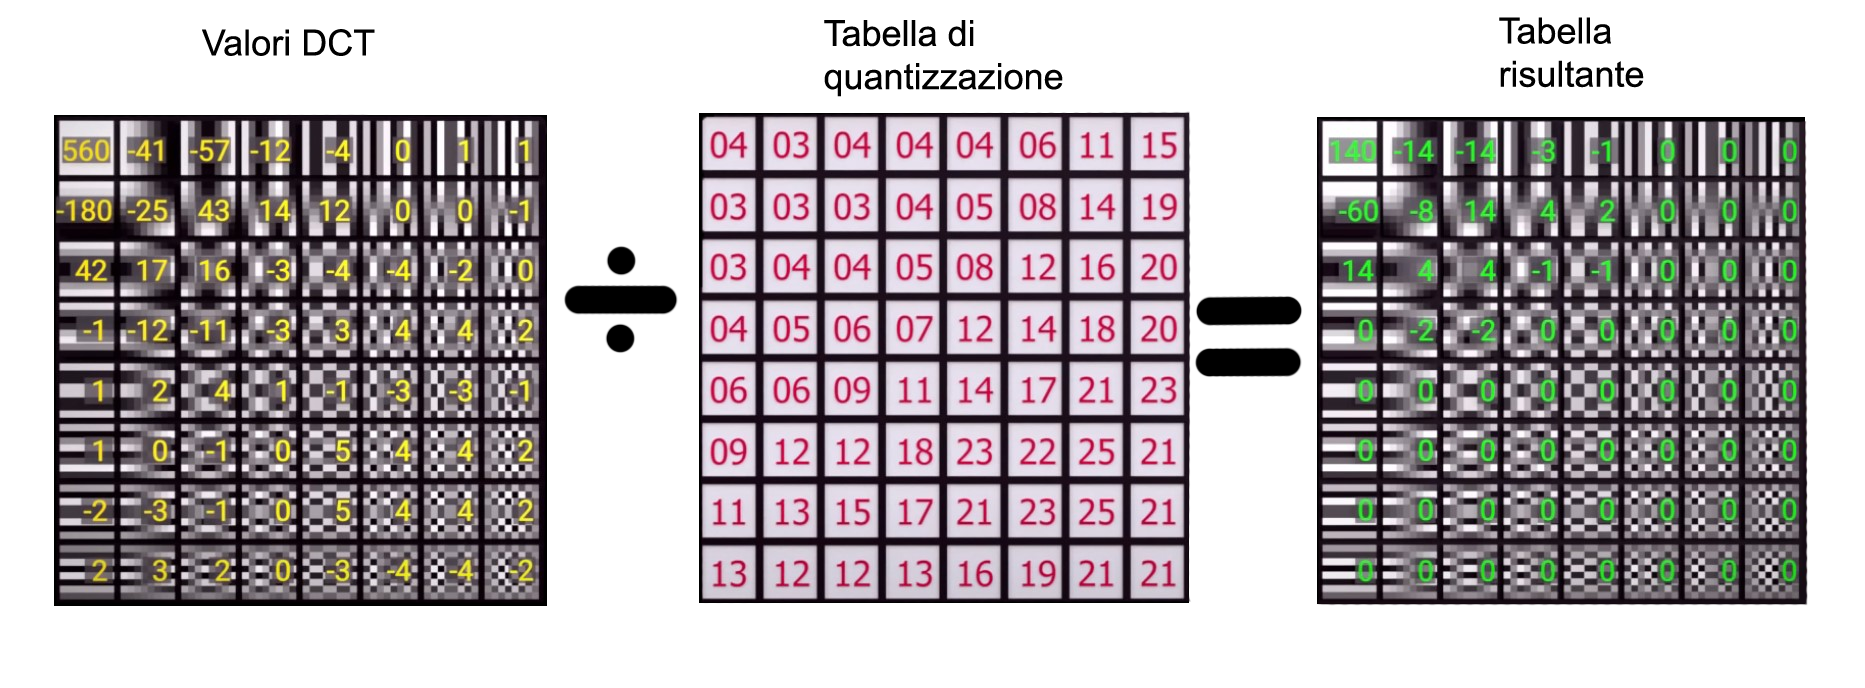
\includegraphics[width=1\textwidth]{images/quantization-example.png}
    \caption{Esempio di quantizzazione della matrice DCT.}
    \label{fig:quantization_example}
\end{figure}

TODO: si potrebbe aggiungere che molti passaggi come gli ultimi due avvengono anche nella compressione delle immagini, come nella jpeg

\paragraph{Entropy Coding}\hphantom{A}\\
Nella fase di Entropy Coding, si mira a comprimere ulteriormente i dati, facendo riferimento non
all'immagine come tale, ma come ad una stringa di bit o simboli. Esistono diversi tipi di
algoritmi di Entropy Coding che possono variare da codec a codec e da implementazione a implementazione.
Tra i più importanti vi è l'\textbf{Arithmetic codec}, il quale cerca di predire i prossimi
simboli o bit in base a una serie data di simboli e una tabella di probabilità. Durante ogni fase
della codifica di un video, viene applicato un algoritmo di codifica diverso o leggermente
modificato. Un altro algoritmo di codifica degno di nota è il \textbf{codifica di Huffman}, o
Huffman encoding, rinomato per la sua flessibilità. Oltre ad essere utilizzato nella codifica video,
trova impiego anche nella codifica delle immagini (come nella JPEG), nella codifica audio
(come nella MP3) e nella compressione dei file (come nei formati PKZIP, ZIP e WinRar).

Nella codifica video, la \textbf{codifica di Huffman} subisce leggere modifiche e viene impiegata
in combinazione con l'algoritmo \textbf{Run Length}. Quest'ultimo viene viene applicato alle matrici
quantizzate, come discusso nel paragrafo precedente. In questo contesto, i valori delle matrici vengono
letti in modo zig-zag, partendo dall'angolo in alto a sinistra e procedendo verso il basso a destra.
Questo schema di lettura organizza i valori in modo tale che quelli con frequenza più alta, spesso 
rappresentati da sequenze di zeri consecutive, si trovino verso la fine della sequenza. Una volta ottenuta
la lista di numeri, quando si incontrano due o più numeri ripetuti si tiene conto di quante volte un certo
numero si è ripetuto invece di riscrivere ogni volta lo stesso numero (vedi l'esempio della
Figura~\ref{fig:huffman_example})).

\begin{figure}[h]
    \centering
    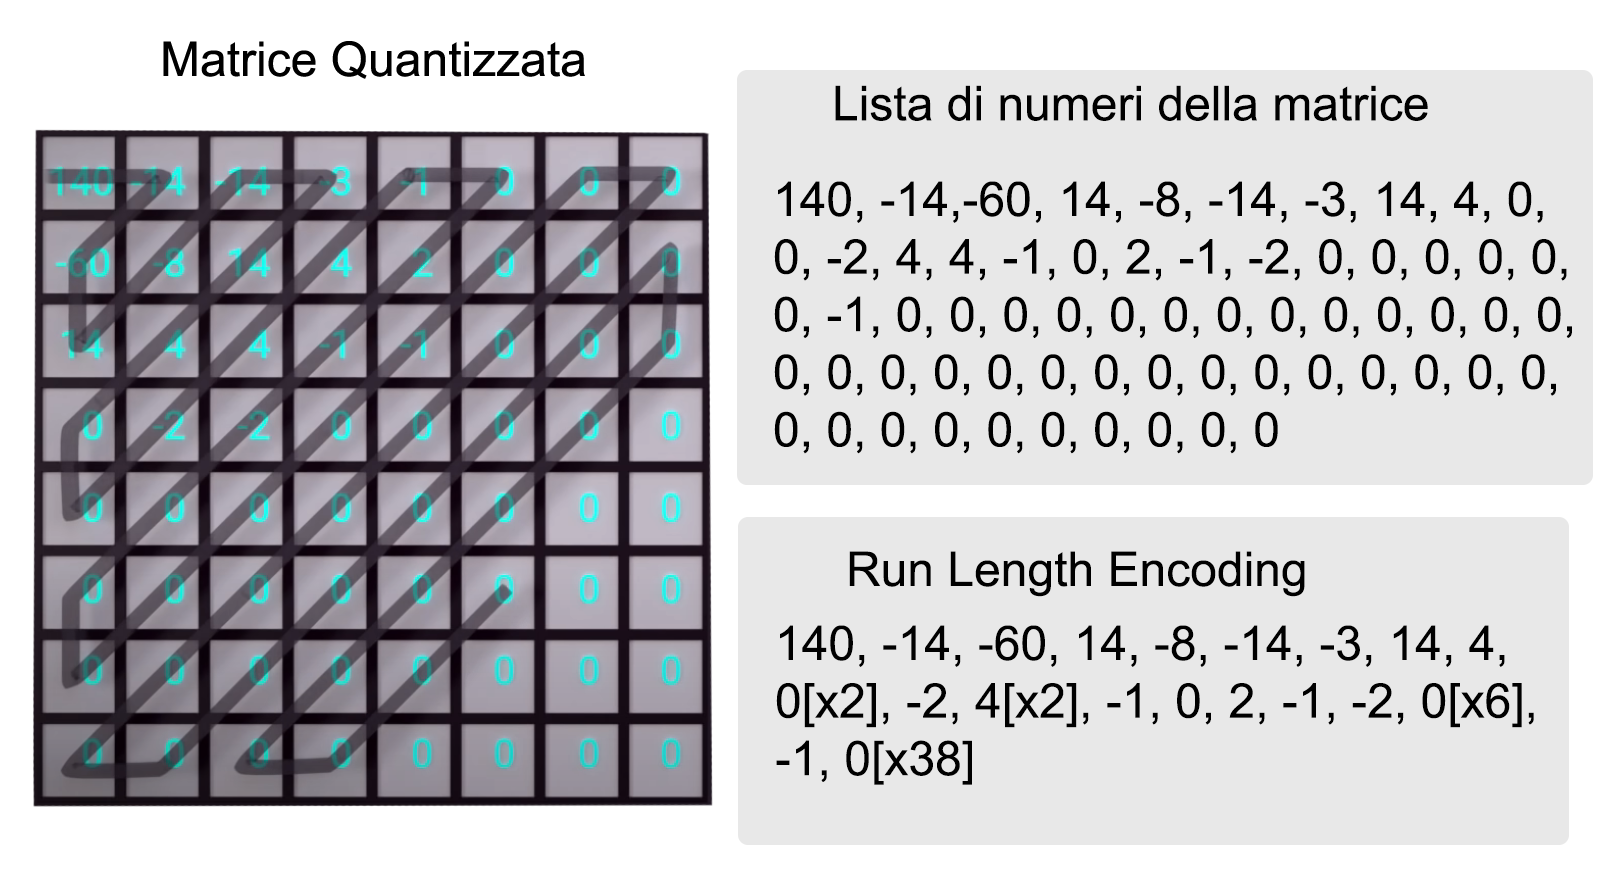
\includegraphics[width=1\textwidth]{images/huffman-example.png}
    \caption{Esempio della codifica di Huffman e Run Length.}
    \label{fig:huffman_example}
\end{figure}

Una volta ottenuta una lista con tutti i numeri e la loro frequenza, possiamo procedere applicando
la \textbf{codifica di Huffman} (nota come in questo paragrafo verrà spiegato come l'algoritmo
viene applicato alla codifica video, se interessati ad una visione più ampia,
\href{https://www.youtube.com/watch?v=JsTptu56GM8}{questo video} lo spiega nel dettaglio con tanto
di illustrazioni). L'algoritmo è diviso in diversi passaggi:

\begin{enumerate}
    \item Si ordinare la lista precedentemente ottenuta in base alla frequenza dei simboli.
    \item Si prendono gli ultimi due elementi e si inizia a costruire un piccolo albero con a base i due
    elementi selezionati e come padre la somma di tutti i figli.
    \item Si prende l'oggetto albero appena creato e lo si reinserisce nella lista nella posizione dettata
    della propria frequenza.
    \item Si procede in questo modo fino a quando la lista sarà composta da un solo elemento.
\end{enumerate}

\begin{figure}[h]
    \centering
    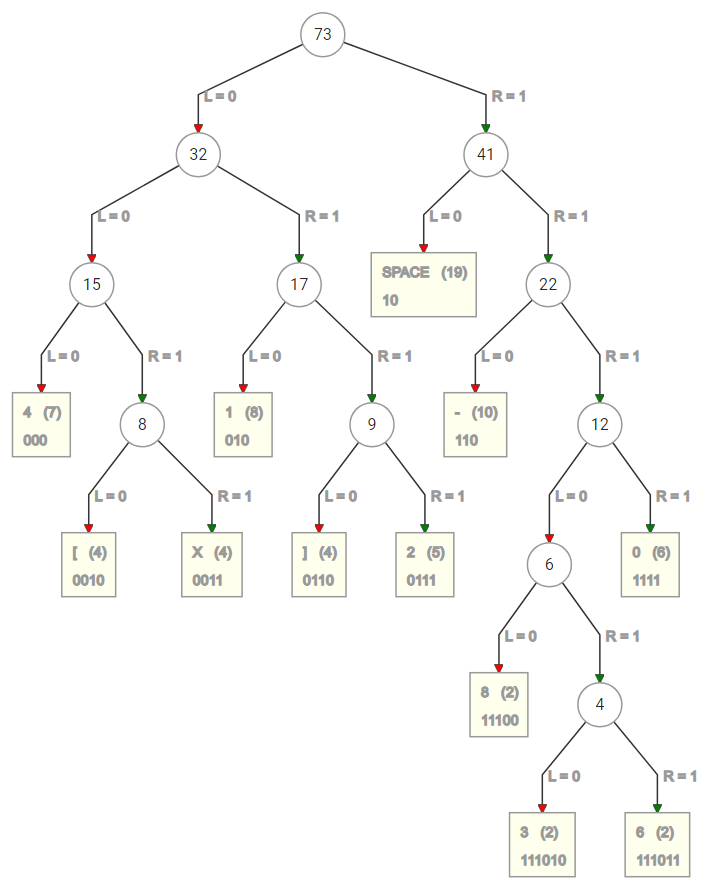
\includegraphics[width=0.8\textwidth]{images/huffman-tree.png}
    \caption{Esempio di un albero di Huffman costruito con i valori ottenuti grazie all'algoritmo
    Run Length.}
    \label{fig:huffman_tree}
\end{figure}

A questo punto, si dispone di un vasto albero che contiene tutti i numeri della lista insieme alle
rispettive frequenze (consultare la Figura~\ref{fig:huffman_tree}). Ora, per codificare ciascun numero,
che ricordiamo variare da -127 a 128, non è più necessario utilizzare 8 bit, ma in molti casi molto
meno. Abbiamo trasformato il processo di codifica da una rappresentazione binaria diretta di ciascun
numero a un'indicazione degli indici dell'albero, dove ogni sequenza di 0 e 1 determina la direzione
da seguire nell'albero per raggiungere il simbolo desiderato.

Prendendo in considerazione l'esempio illustrato nella Figura~\ref{fig:huffman_example}, inizialmente
la matrice occupava uno spazio di 8x8x8, equivalenti a 512 bit. Dopo l'applicazione degli algoritmi
Run Length e Huffman, il consumo di spazio si riduce drasticamente a soli 239 bit, permettendo un
risparmio di circa il 46\% dello spazio.

\paragraph{Loop filter}\hphantom{A}\\

\paragraph{Ricapitolando}\hphantom{A}\\

La compressione e, soprattutto, la decodifica in tempo reale di un video richiedono considerevole potenza
di calcolo. Il formato H.264 è stato uno dei primi codec a necessitare di un acceleratori hardware
dedicati per la decodifica dei video, poiché le operazioni computazionali richieste diventavano sempre
più complesse. Questo portò alla luce che con l'avanzare delle nuove tecnologie per la compressione dei
video, che riducevano le dimensioni dei file, aumentava anche la potenza di calcolo necessaria per la
codifica e decodifica dei video.

Le differenze principali con il codec H.261 sono

- supporto di più dimensioni per la chroma subsampling
- slice di dimensioni variabili, quanto nel vecchio codec ogni slice aveva una dimensione prefissata
- supporto a DVD, ATV, HDTV
- i motion vector non sono più limitati a spostare i macroblocks all'interno della loro griglia
(ovvero che un macroblock deve per forza stare al posto di un altro), ma possono anche indicare una
posizione con una precisione di 1/4 di macroblock.
- predizione dei movimenti  (da controllare)
- la trasformazione discreta del coseno (DCT)
- la compensazione del movimento (da controllare)

Introduce la possibilità di codificare fino a 4k, poi più avanti arriva fino all'8k.
Youtube lo ha usato fino al 2010 per poi abbandonarlo in favore del proprio VP8.
TODO: L'h264 essendo una tecnica che racchiude molti algoritmi complessi per la compressione video, necessita di accelleratori hardware per poter decodificare i fotogrammi in tempo reale.

\subsection{H.265}
Fino a 8K
\subsection{VP9}    % forse non serve descriverlo
\subsection{AV1}
TODO: il codec AV1 è molto lento nel codificare/decodificare video, ma con un acceleratore apposito è nettamente più veloce del H.265

\subsection{Comparazione delle prestazioni}

\section{Vantaggi per le aziende}

\section{Sfide e considerazioni}
Non dimenticare di discutere anche delle sfide e delle considerazioni pratiche legate all'adozione di nuovi codec, come il supporto hardware/software, la compatibilità con dispositivi esistenti e la gestione dei diritti d'autore.

\section{Conclusioni}
TODO: si potrbbe parlare dell'approccio di NVIDIA per le video chat.

\section{Bibliografia}
\\+sito che parla della storia degli encorder https://api.video/blog/video-trends/the-history-of-video-compression-starts-in-1929/
\\+parla dei tecnicismi del h.261 https://users.ece.utexas.edu/~ryerraballi/MSB/pdfs/M4L2.pdf
\\+bitrate https://it.wikipedia.org/wiki/Velocit%C3%A0_di_trasmissione
\\+utile! parla dei tecnicismi del h.264 nella sezione di Implementing h.264 https://www.embedded.com/implementing-h-264-video-compression-\\algorithms-on-a-software-configurable-processor/
\\+utile! intra prediction https://www.sciencedirect.com/topics/computer-science/intra-prediction
\\+utile! sito di International Telecommunication Union che parla dello standard h.264 https://www.itu.int/rec/T-REC-H.264-202108-I/en
\\+repository di un'implementazione dell'h.264 https://github.com/cisco/openh264
\\+parla di molte cose... vechi codec, tranformation, quantizzazione https://www.researchgate.net/publication/334546287_Data_Reduction_in_MMBD_Computing#pf17
\\+codifica di huffman https://en.wikipedia.org/wiki/Huffman_coding
\\+sito utilizzato per costruire l'albero di huffman https://suhaan-bhandary.github.io/Huffman-Coding/
\\-sito ufficiale di h.265 https://hevc.hhi.fraunhofer.de/
\\+repository di h.265 https://vcgit.hhi.fraunhofer.de/jvet/HM
\\-utile! parla dei tecnicismi del h.265 nella sezione di Coding tools https://en.wikipedia.org/wiki/High_Efficiency_Video_Coding
\\-utile! paragona AV1 a h.265 https://subclassy.github.io/compression#:~:text=265%20takes%202.83s%20on,so%20much%20time%20to%20process.
\\-utile! paragona le performance dei vari codec su hw nvidia https://developer.nvidia.com/video-codec-sdk
\\-utile! https://support.google.com/youtube/answer/2853702?hl=it

\end{document}
